\documentclass[11pt]{article}
\usepackage[margin=0.8in]{geometry}
\usepackage{graphicx}
\usepackage{amsmath}
\usepackage{amssymb}
\usepackage{hyperref}
\usepackage[numbers]{natbib}
\usepackage{enumitem}
\usepackage{booktabs}
\usepackage{float}
\usepackage{microtype}
\usepackage{caption}
\usepackage{subcaption}
\captionsetup{font=small, skip=4pt}
\setlength{\parskip}{0.25em}
\setlist{itemsep=0.1em, topsep=0.15em, parsep=0pt}

\begin{document}
\thispagestyle{empty}

\begin{center}
	\rule{\linewidth}{1mm} \\[0.2cm]
	{ \Large \bfseries ISyE 6644 - Simulation, Summer 2026 \\[0.1cm]
		Final Report}\\[0.2cm]
	\rule{\linewidth}{1mm} \\[0.15cm]
\end{center}

\noindent\textbf{Project Topic Number:} 18 \quad
\textbf{Project Group Number:} 132 \\
\textbf{Team Members:} Ahmadou Diallo (adiallo41) (solo group) \\
\textbf{Project Title:} A Monte Carlo Simulation Laboratory for the Newsvendor Problem

\section*{Abstract}
The newsvendor problem is the canonical single-period inventory model: choose an order quantity
$Q$ before observing stochastic demand $D$, trading the cost of ordering too little against the
cost of ordering too much. This project builds a Monte Carlo engine that estimates expected
profit across a grid of candidate order quantities, validates the simulated optimum against the
closed-form critical-ratio solution $F(Q^*) = c_u/(c_u+c_o)$, and wraps the engine in an
interactive Streamlit application so a user can vary prices, costs, and demand assumptions and
immediately see updated results. Across five demand distributions (Normal, Uniform, Poisson,
Lognormal, Gamma) calibrated to comparable means and variances, the simulated optimum matched the
analytical optimum to within 0.23\% using 50{,}000 replications, and the running-mean profit
estimate visibly stabilized well before that replication count. A sensitivity analysis further
shows the optimal order quantity is far more responsive to the underage/overage cost ratio than
to demand variability, and that the \emph{shape} of the demand distribution shifts the optimum
even when the critical ratio is held fixed.

\section*{Background \& Description of the Problem}
Any retailer or single-run producer who must commit to inventory before demand is known faces the
same trade-off: order too little and lost sales are forfeited; order too much and the surplus
must be discounted or salvaged. This is the newsvendor (newsboy) problem, one of the oldest models
in inventory theory, applicable wherever a single ordering decision precedes a single uncertain
selling season --- fashion apparel, holiday merchandise, fresh produce, or even cloud-capacity
decisions made before demand materializes.

Let $D$ be demand, $Q$ the order quantity, $p$ the price, $c$ the unit cost, and $s$ the salvage
value per leftover unit ($s<c<p$). Realized profit for demand outcome $d$ is
\[
\pi(d, Q) = p \cdot \min(d, Q) + s \cdot \max(Q - d, 0) - c \cdot Q - g \cdot \max(d - Q, 0),
\]
where $g \geq 0$ is an optional goodwill penalty per unit of unmet demand. Differentiating
$\mathbb{E}[\pi(D,Q)]$ with respect to $Q$ gives the textbook critical-ratio condition
\[
F(Q^*) = \frac{c_u}{c_u + c_o}, \qquad c_u = p - c + g \;\;(\text{underage cost}), \qquad
c_o = c - s \;\;(\text{overage cost}),
\]
where $F$ is demand's CDF. This closed form is the benchmark used throughout to check the
simulation for correctness: a correctly implemented Monte Carlo engine should estimate an optimal
$Q$ that converges to $F^{-1}(c_u/(c_u+c_o))$.

This is a \emph{programming-oriented} project: the goal was to design, build, and document a
working simulation tool, show its output is statistically correct via convergence and validation
checks, and package it as an interactive application usable without a simulation background. The
Main Findings section below covers the engine and app, validation against the closed form, a
cross-distribution comparison, and a sensitivity analysis, followed by Conclusions.

\section*{Main Findings}

\subsection*{Simulation engine and interactive application}
The engine (\texttt{newsvendor.py}) supports five demand distributions --- Normal, Uniform,
Poisson, Lognormal, Gamma --- each with a sampler and an exact inverse-CDF used both to size the
order-quantity search grid and to compute the analytical $Q^*$. Its core is a vectorized profit
function: given $n$ sampled demands and $m$ candidate order quantities, it returns the full
$n\times m$ matrix of realized profits in one NumPy broadcast rather than looping over $Q$. This
also implicitly applies \textbf{common random numbers} --- the same $n$ demands are reused across
every candidate $Q$ in a run --- so the estimated profit curve is smooth in $Q$ and its argmax is
a far more reliable estimate of $Q^*$ than independently resampling at each grid point would give.
For a grid spanning the 0.5th--99.5th demand percentile, the engine reports at every point the
mean simulated profit, a 95\% confidence interval ($\pm1.96\cdot\mathrm{SE}$), and the empirical
service level $P(D\le Q)$; the simulated optimum $\hat{Q}^*$ is the grid's argmax.

The engine is wrapped in a Streamlit app (\texttt{app.py}) meeting the brief's ``pretty and
interesting to use'' requirement with a real, runnable tool. All economic inputs (price, cost,
salvage, an optional stockout penalty), the demand distribution and parameters, replication
count, grid resolution, and random seed are adjustable from a sidebar, and every chart recomputes
live (cached for repeated inputs). Four tabs organize the output: \textbf{Profit vs.\ order
quantity} (the expected-profit curve with its confidence band and both optima marked, Figure
\ref{fig:row1}a), \textbf{Profit distribution} (a histogram at a user-chosen $Q$, Figure
\ref{fig:row2}a), \textbf{Sensitivity analysis} (a heatmap of optimal $Q$ vs.\ cost and demand
variability, Figure \ref{fig:row2}b), and \textbf{Methodology \& validation} (equations, a
simulated-vs.-analytical table, and a convergence plot, Figure \ref{fig:row1}b). All figures
below are produced by the same engine via \texttt{generate\_figures.py}, so every number is
reproducible by re-running that script or the app with the same seed.

\subsection*{Validation against the closed-form solution}
The baseline scenario is $p=\$25$, $c=\$12$, $s=\$5$, demand $\sim \mathcal{N}(200,40^2)$, giving
$c_u=13$, $c_o=7$, critical ratio $0.65$. With a 150-point grid and $n=50{,}000$ replications per
point (seed 42):

\begin{table}[H]
\centering
\small
\begin{tabular}{lcc}
\toprule
 & Order quantity & Expected profit \\
\midrule
Analytical $Q^*$ (critical ratio) & 215.4 & \$2{,}302 \\
Simulated $\hat{Q}^*$ (grid argmax) & 215.9 & \$2{,}303 \\
\bottomrule
\end{tabular}
\caption{Simulated vs.\ closed-form optimum, baseline scenario. Gap: 0.23\%.}
\label{tab:validation}
\end{table}

\begin{figure}[H]
\centering
\begin{minipage}{0.48\textwidth}
\centering
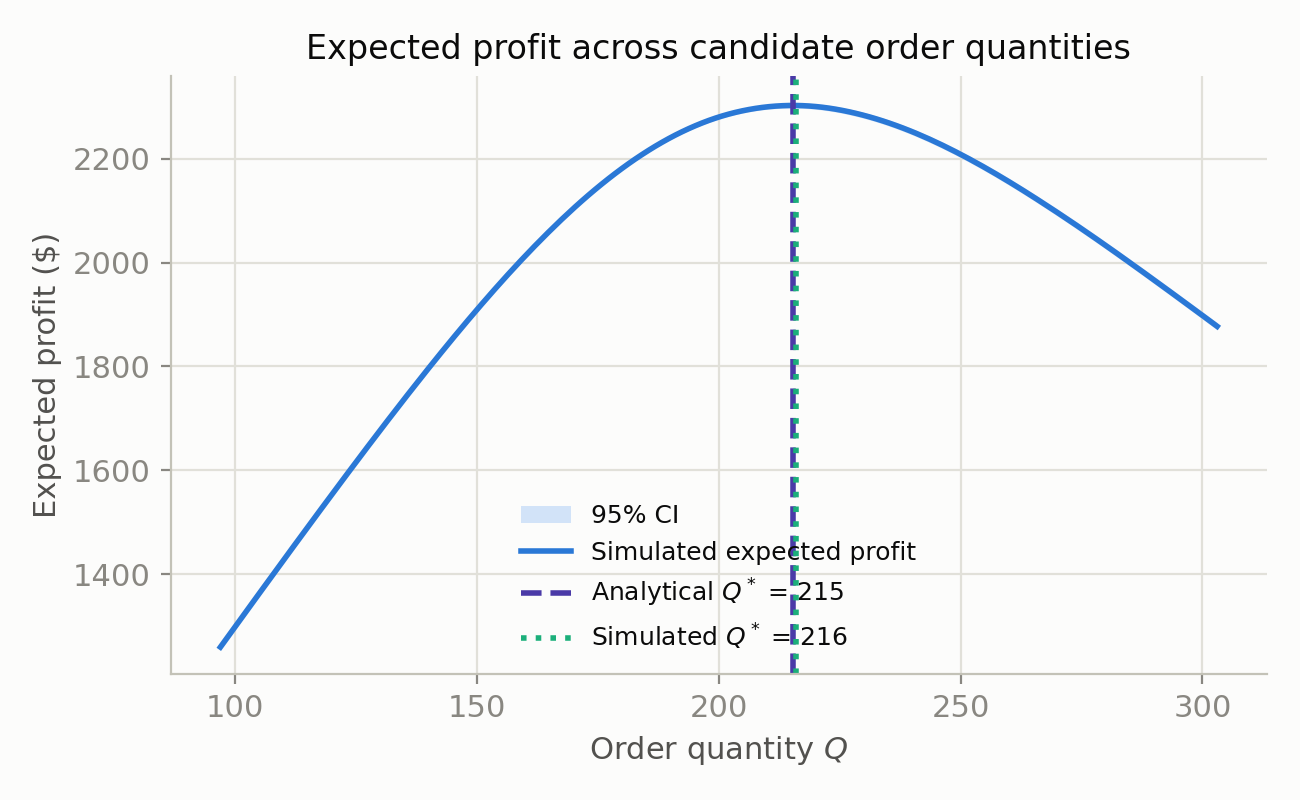
\includegraphics[width=\textwidth]{figures/fig_profit_curve.png}
\subcaption{Expected profit vs.\ order quantity, with both optima marked --- visually
indistinguishable, consistent with the 0.23\% gap in Table~\ref{tab:validation}.}
\end{minipage}\hfill
\begin{minipage}{0.48\textwidth}
\centering
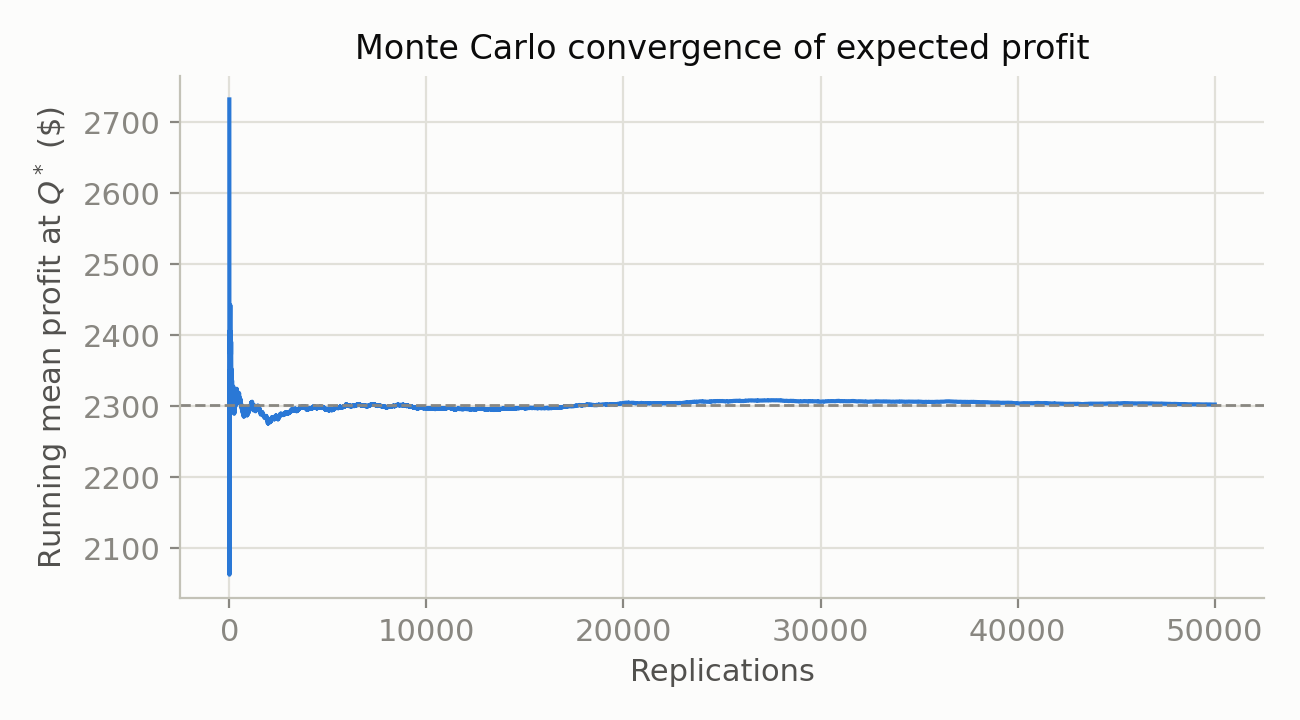
\includegraphics[width=\textwidth]{figures/fig_convergence.png}
\subcaption{Running-mean profit at $\hat{Q}^*$ vs.\ replications. It stabilizes well before
10{,}000 replications, the expected $O(1/\sqrt{n})$ behavior.}
\end{minipage}
\caption{Optimization and convergence, baseline scenario ($n=50{,}000$).}
\label{fig:row1}
\end{figure}

\subsection*{Profit distribution and sensitivity}
The full profit distribution at $\hat{Q}^*\approx216$ (Figure~\ref{fig:row2}a) is left-skewed with
a sharp mass point near the maximum attainable profit $(p-c)\hat{Q}^*\approx\$2{,}808$: whenever
demand meets or exceeds $Q$, every unit sells at full margin regardless of how far demand exceeds
$Q$, so those outcomes collapse onto one bin; below $Q$, profit falls off linearly with the
shortfall. This is a structural property of the newsvendor payoff, and it shows why the mean
profit alone (the closed-form output) can understate the downside risk at a given $Q$.

Figure~\ref{fig:row2}b sweeps unit cost $c$ (which moves the critical ratio, since $c_u=p-c$ and
$c_o=c-s$ both depend on it) against a demand-variability multiplier. $Q^*$ moves far more with
cost than with variability: near baseline, $Q^*$ ranges from about 90 (near the salvage floor) to
past 300 (near the selling price) as $c$ varies, while sweeping variability alone from half to
double the baseline spread moves $Q^*$ comparatively little. This follows directly from the
critical-ratio formula: $c$ has a first-order effect on $F(Q^*)$ itself, while variability only
rescales the response to a \emph{given} ratio --- so getting cost and margin inputs right matters
more than pinning down the demand variance exactly.

\begin{figure}[H]
\centering
\begin{minipage}{0.48\textwidth}
\centering
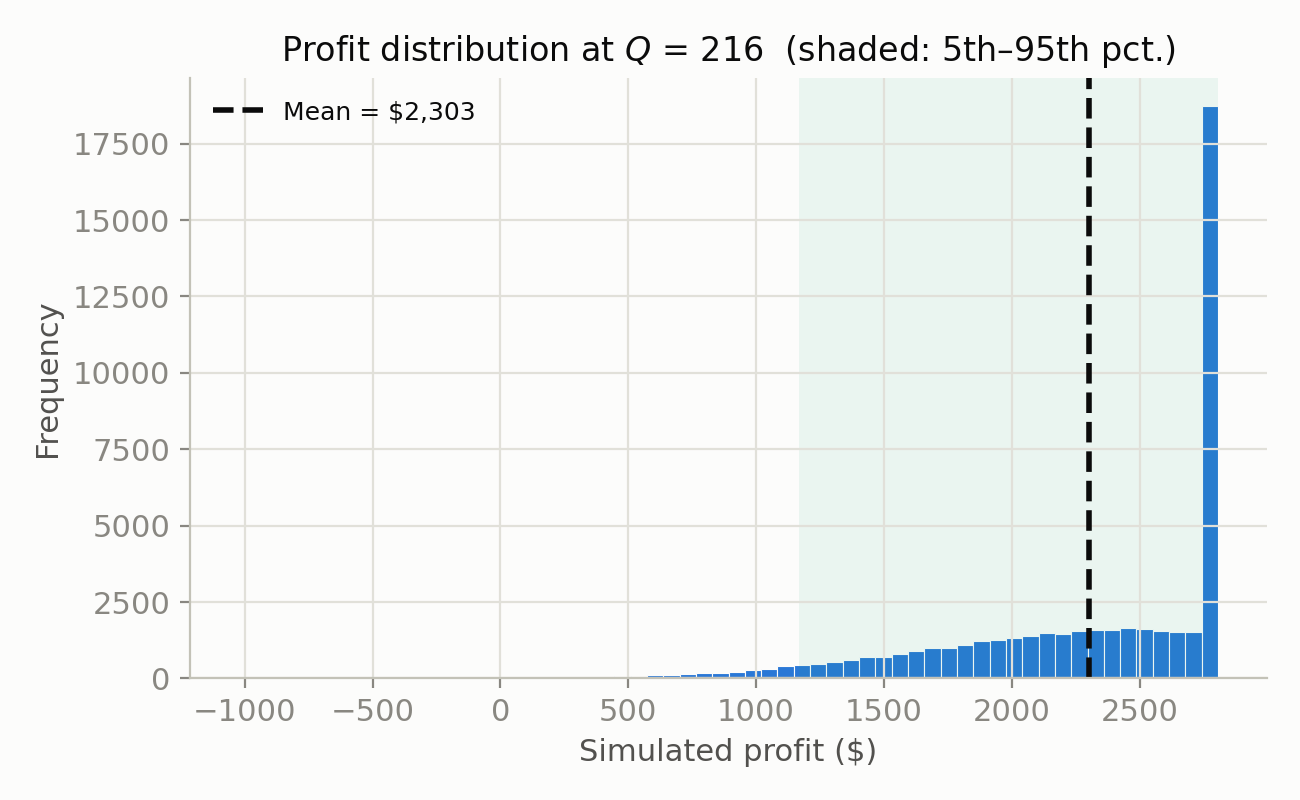
\includegraphics[width=\textwidth]{figures/fig_profit_hist.png}
\subcaption{Simulated profit distribution at $Q=\hat{Q}^*\approx216$ (shaded: 5th--95th pct.).}
\end{minipage}\hfill
\begin{minipage}{0.48\textwidth}
\centering
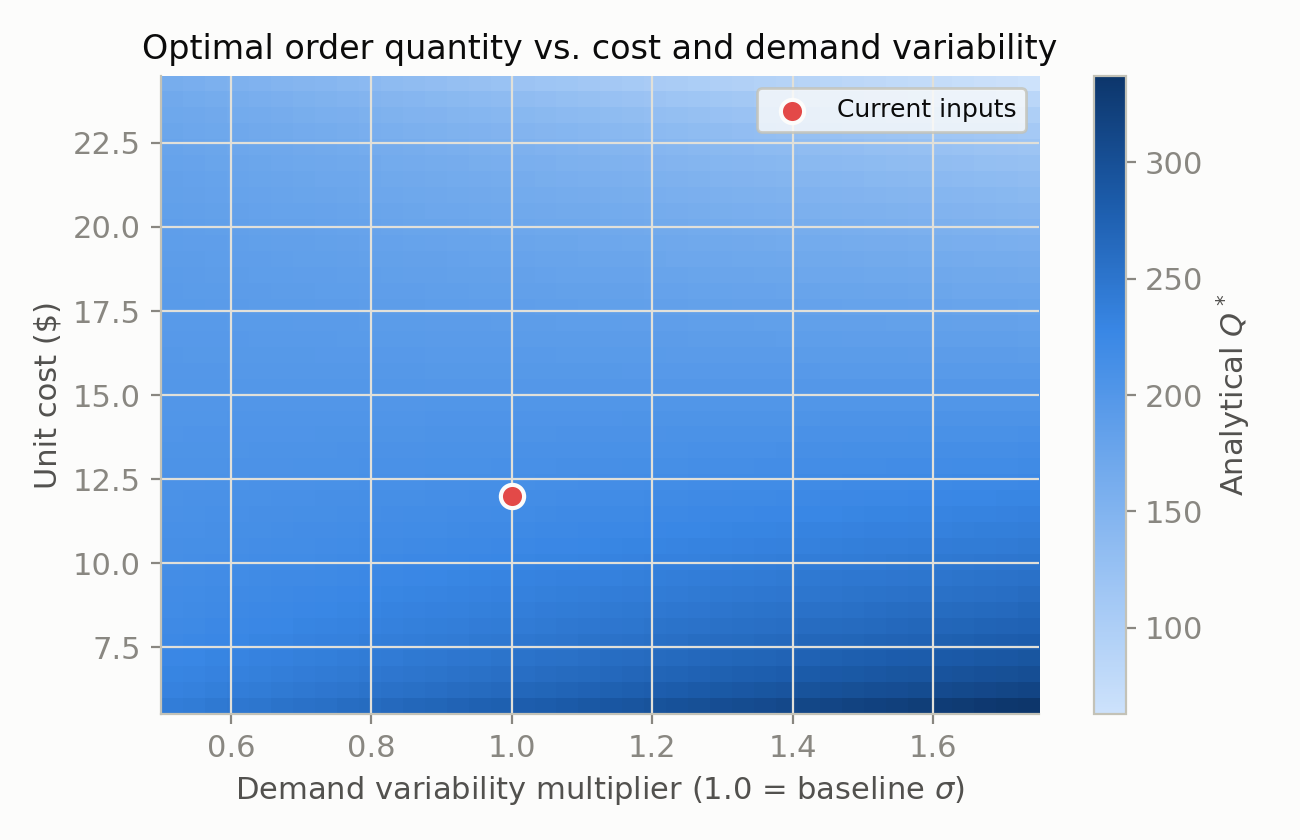
\includegraphics[width=\textwidth]{figures/fig_sensitivity_heatmap.png}
\subcaption{Analytical $Q^*$ vs.\ unit cost and demand-variability multiplier. Red marker:
baseline inputs.}
\end{minipage}
\caption{Risk and sensitivity, baseline scenario.}
\label{fig:row2}
\end{figure}

\subsection*{Cross-distribution comparison}
Table~\ref{tab:crossdist} calibrates all five supported distributions to demand mean 200 and
(where the family allows it) std.\ dev.\ 40, at the same critical ratio 0.65, and reports the
closed-form and simulated $Q^*$ for each.

\begin{table}[H]
\centering
\small
\begin{tabular}{lccccc}
\toprule
Distribution & Analytical $Q^*$ & Simulated $\hat{Q}^*$ & Gap & $\mathbb{E}[\pi(\hat{Q}^*)]$ & Demand std.\ dev. \\
\midrule
Normal & 215.4 & 215.9 & 0.23\% & \$2{,}303 & 40.1 \\
Uniform & 220.8 & 220.7 & 0.03\% & \$2{,}287 & 40.0 \\
Poisson & 205.0 & 205.1 & 0.05\% & \$2{,}495 & 14.1 \\
Lognormal & 211.7 & 211.7 & 0.00\% & \$2{,}296 & 40.1 \\
Gamma & 213.0 & 212.9 & 0.07\% & \$2{,}295 & 40.2 \\
\bottomrule
\end{tabular}
\caption{Optimal order quantity across demand distributions, mean 200, std.\ dev.\ 40 where
permitted, critical ratio 0.65 ($n=50{,}000$, seed 42).}
\label{tab:crossdist}
\end{table}

The gap stays below 0.25\% across every family tested, including discrete Poisson and the two
skewed continuous families --- correctness does not depend on demand being Normal or continuous.
Holding the critical ratio and first two moments fixed, \textbf{$Q^*$ still varies by about 16
units (215 vs.\ 221) across distribution shapes}, since $F^{-1}(0.65)$ depends on more than mean
and variance. Poisson is a special case: its variance is tied to its mean ($\sigma^2=\lambda$), so
it cannot be calibrated to std.\ dev.\ 40 at mean 200 (its actual std.\ dev.\ is
$\sqrt{200}\approx14.1$); its lower $Q^*$ and higher profit mainly reflect lower relative demand
uncertainty, not a shape effect.

\section*{Conclusions}
Both project goals --- a validated Monte Carlo engine and an interactive tool built on it --- were
met with results statistically checked rather than assumed. (1) A vectorized, common-random-numbers
grid search reproduces the closed-form optimum to within a quarter of a percent across five
distributions, including discrete and skewed families. (2) The convergence plot shows the
expected-profit estimate stabilizes well within the replication budgets used, so reported optima
are not sampling noise. (3) Demand-distribution \emph{shape} --- not only its mean and variance ---
shifts the optimal order quantity at a fixed critical ratio, a distinction the closed form alone
does not surface. (4) The optimal order quantity is considerably more sensitive to the
underage/overage cost structure than to demand variability, so effort spent pinning down price,
cost, and salvage assumptions pays off more than refining the demand-variance estimate.

Future work: an empirical (bootstrap) demand option fit to a user-supplied sales history rather
than a named parametric family; a multi-period, correlated-demand extension; and a formal
ranking-and-selection procedure (e.g.\ indifference-zone) so the tool could recommend a best $Q$
with a statistical guarantee rather than a single-run grid argmax.

\end{document}
